\documentclass[12pt]{article}
\setlength{\oddsidemargin}{0in}
\setlength{\evensidemargin}{0in}
\setlength{\textwidth}{6.5in}
\setlength{\parindent}{0in}
\setlength{\parskip}{\baselineskip}

\usepackage{xcolor}
\usepackage{amsmath,amsfonts,amssymb}
\usepackage{qtree}
\usepackage{enumerate}
\usepackage{multirow}
\usepackage{graphicx}
\usepackage{forest}
\usepackage{colortbl}

\begin{document}

CSCI 4448 Spring 2016 \hfill Project Write-up 2\\

\hrulefill
%%%%%%%%%%%%%%%%%%%%%%%%% SECTION 1  %%%%%%%%%%%%%%%%%%%%%%%%%
\begin{center}
  \textbf{Business Requirements} \\
\begin{tabular}{| l | l | l | l | l | }
  \hline
  \textbf{ID}  & \textbf{Requirement} & \textbf{Topic Area} & \textbf{Actor} & \textbf{Priority} \\ \hline
  BR-001 & Ingredients must be able to include sponsor links & Advertising & All & Medium \\ \hline 
  BR-002 & Collect user data for later processing & Reporting & Admin & Medium \\ \hline
  BR-003 & Replication factor of 3 for data consistency & Database & Admin & High \\ \hline

\end{tabular}
\\
  \vspace{1cm}

\begin{center}
  \textbf{Use Case Document}
  \begin{tabular}{ l | l }
    \textbf{User ID} & \textbf{Requirement} \\ \hline \rowcolor[gray]{.95}
    UR-001 & The user can select an ingredient from a category \\ 
    UR-002 & The user can select an ingredient from a search function \\ \rowcolor[gray]{.95}
    UR-003 & The user can filter options based on dietary preference \\ 
    UR-004 & The user can filter options based on price of ingredients \\ \rowcolor[gray]{.95}
    UR-005 & The user can makr a dietary preference as mandatory or prefered \\
    UR-006 & The user can delete ingredients from their list \\ \rowcolor[gray]{.95}
    UR-007 & The user can generate recipes based on current ingredient selection \\ \hline
  \end{tabular}
\end{center}
 \textbf{User Requirements} \\
\begin{tabular}{| l | l | l | l | l | }
  \hline
  \textbf{ID}  & \textbf{Requirement} & \textbf{Topic Area} & \textbf{Actor} & \textbf{Priority} \\ \hline
  UR-001 & Can enter optimal price range per meal & Interface & User & Medium \\ \hline 
  UR-002 & Dietary Restrictions Option  & Interface & User & Medium \\ \hline
  UR-003 & If no matches find next closest & Functionality & User & Low \\ \hline
  UR-004 & Search Bar for ingredient list & Interface & User & High \\ \hline
  UR-005 & Category based ingredient search & Interface & User & High \\ \hline
  UR-006 & Able to remove ingredients after search & Functionality & User & Medium \\ \hline
\end{tabular}
\\
  \vspace{1cm}
  \textbf{Non-Functional Requirements}
\begin{tabular}{| l | l | l | l | l | }
  \hline
  \textbf{ID}  & \textbf{Requirement} & \textbf{Topic Area} & \textbf{Actor} & \textbf{Priority} \\ \hline
  NFR-001 & Show 10 recipes upon search  &  Interface & User & Low  \\ \hline 
  NFR-002 & Return at least 3 hits in under one second & Media & User &  Medium\\ \hline
  NFR-003 & Less than one second load time for inital website &  Website & All & High \\ \hline
  NFR-004 & Recent database results cached locally & Database & User & Low \\ \hline
  NFR-005 & Set partition size for Database & Database & Admin & Low \\ \hline

\end{tabular}
\end{center}
\begin{center}
\begin{figure}
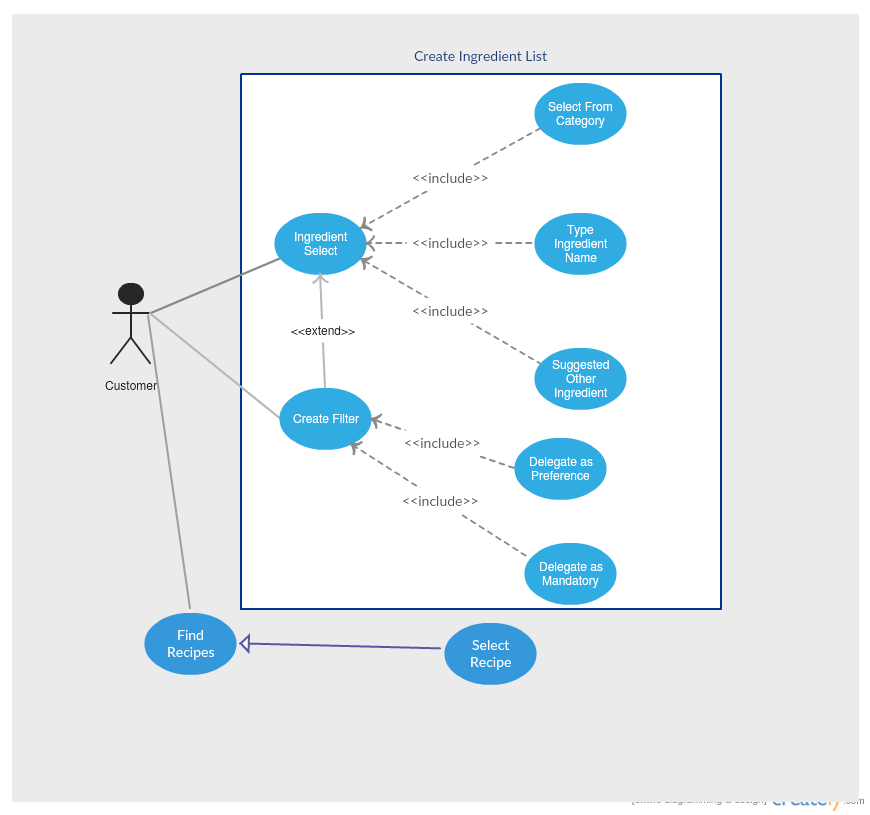
\includegraphics[width=\linewidth]{UseCase.png}
\caption{Use Case.}
\label{fig:UseCase}
\end{figure}
\end{center}
\newpage
\begin{center}
  \textbf{Data Storage}
\end{center}
\textit{Database: } We will be using Cassandra DB so that we can easily delegate multi-factor replication and partition management. We will be hosting our database using
Amazon S3 which easily integrates a Cassandra deployment. \\
\vspace{1cm} \\
\textit{Data Persistance: } We will have a static list of recipe names with ingredients lists which will persist. We will query the database and MapReduce based on the ingredients
provided by the user to provide a list of the 10 best matches. We will have a separate partition of data persistance allocated for user ingredients data. 

\newpage
\begin{center}
  \textbf{Class Diagram}
\end{center}

\end{document}
